


With the rapid growth of e-commerce, new products are increasingly introduced into the market place on a daily basis.  A larger subset of these products consists of our daily needs or off-the-shelf products (Table~\ref{tab:ebay-standard-products}), while a much smaller subset can be attributed as {\em unique}, {\em creative}, {\em serendipitous}, or {\em interesting} (Table~\ref{tab:ebay-interesting-products}). The latter class of products often provokes an emotive response in users and gives them a more engaging experience. Automatic discovery of this type of products is an important problem in e-commerce for creating an engaging experience for the users and encouraging them to return to the site for a much more pleasing shopping experience. Quantifying interestingness, however,  is a challenging problem for several reasons. First, the notion of interestingness is not very well understood and is very subjective. We only understand certain dimensions of interestingness, such as visual appeal in images, or humor in the text domain, among other dimensions. Second, interestingness is very subjective. However, we believe that there still exists a class of products that appear interesting to a sufficiently large population of users (see sites such as {\em Pinterest\footnote{\url{www.pinterest.com}}}, for example). Identifying such products and surfacing them to the users plays an important role for generating a different form of engagement in e-commerce sites. 

In this paper we present an information theoretic approach for quantifying certain dimensions of text interestingness (where it can be subsequently used to measure an interestingness score for e-commerce products based on the product titles, for example). We hypothesize that many interesting text forms (e.g., a product title in e-commerce) often present diversity in terms of the text describing them. For example, consider the products shown in the Table~\ref{tab:ebay-standard-products}. For each product, all the keywords observed in the title are expected to be seen together and thus offer less diversity in terms of the topics they represent. However, in the examples shown in Table~\ref{tab:ebay-interesting-products}, the highlighted keywords offer the largest diversity in each case. In other words what makes these products textually interesting is the juxtaposition of keywords that one does not normally expect to see them co-occur in a categorical text document. As an example, in Figure~\ref{tab:ebay-interesting-products}(a), in the context of iPhone cases, one would not expect to observe topics that relate to makeup. Based on this hypothesis we introduce an information-theoretic approach for measuring topic diversity based on {\em Jensen-Shannon Diversity} and show how it correlates with text interestingness. First we show how to build a word-to-topic distributional model by learning an LDA~\cite{Blei:2003:LDA:944919.944937}, trained over a corpus of documents. Next, we introduce several techniques for improving the base model that smoothes the distributions based on topic similarities and keyword sailiency. Finally, we show how such a distributional model can be used to measure {\em Jensen-Shannon Diversity} for a given text. We also present results evaluating the performnce of our diversity metric in two different real world domains: (1) identifying interesting eBay products based on the diversity in their titles; (2) idenitifying the most diverse National Science Foundation Scholarship proposal abstracts (introduced in~\cite{bache:2013}). 

The rest of this paper is organized as follows. In Section~\ref{sec:related-work} we briefly overview the related work. In Section~\ref{sec:information-diversity} we introduce {\em Jensen-Shannon Diversity} and discuss an approach for building a text model suitable for this metric. In Sections~\ref{sec:the-readers-model} and \ref{sec:topic-similarities} we present a set of enhancements to the base model. In Section~\ref{sec:experiments} we present our results in two different sets of experiments. We first evaluate our approach in an unsupervised setting and present our main results in terms of a set of ROC curves. We also present results in a supervised setting where we show how a model learned using text diversity features compares to several other text classification models. We finalize the paper by presenting some concluding remarks in Section~\ref{sec:conclusions}.

\begin{table*}[t]
\caption{Examples of eBay off-the-shelf products. Note that in every case, the word occurrences in the titles match our expectation.}
\label{tab:ebay-standard-products}
\begin{center}
\begin{tabular}{LLL}
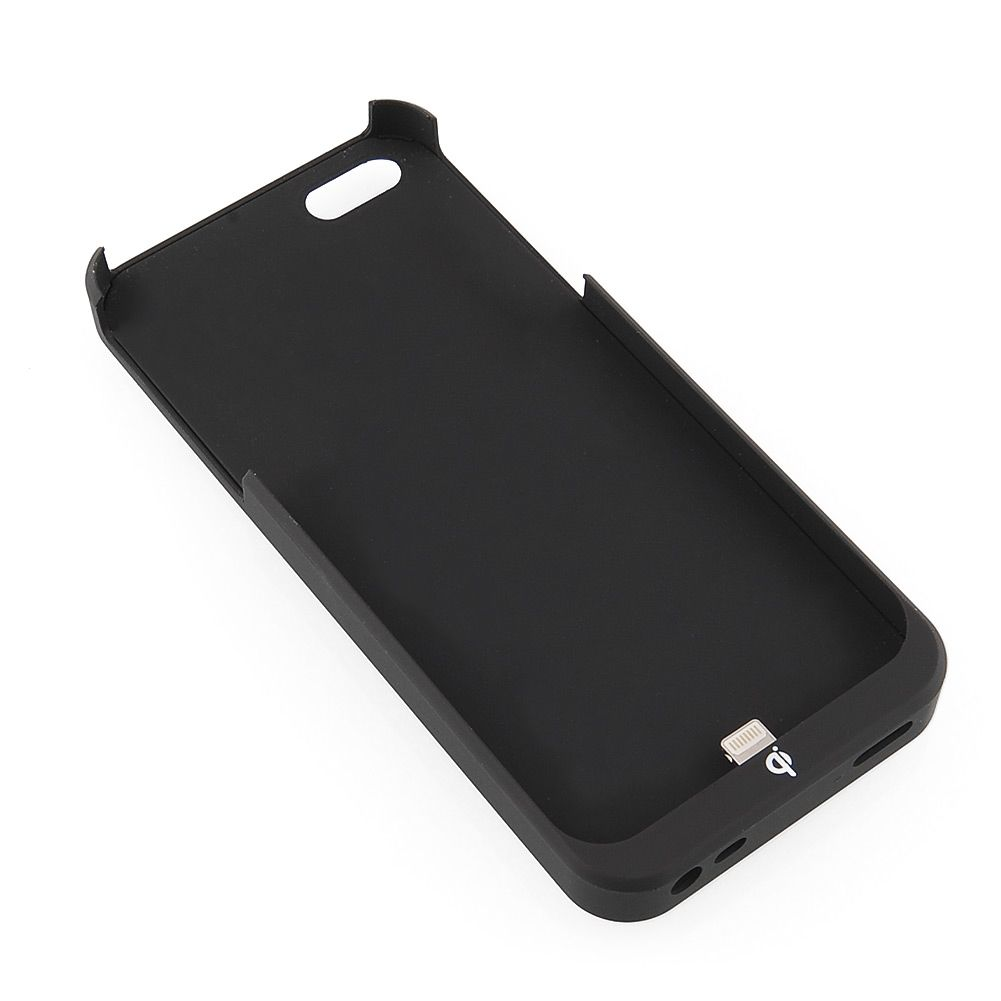
\includegraphics[height=4.0cm]{figures/standard-iphone-case.jpg}&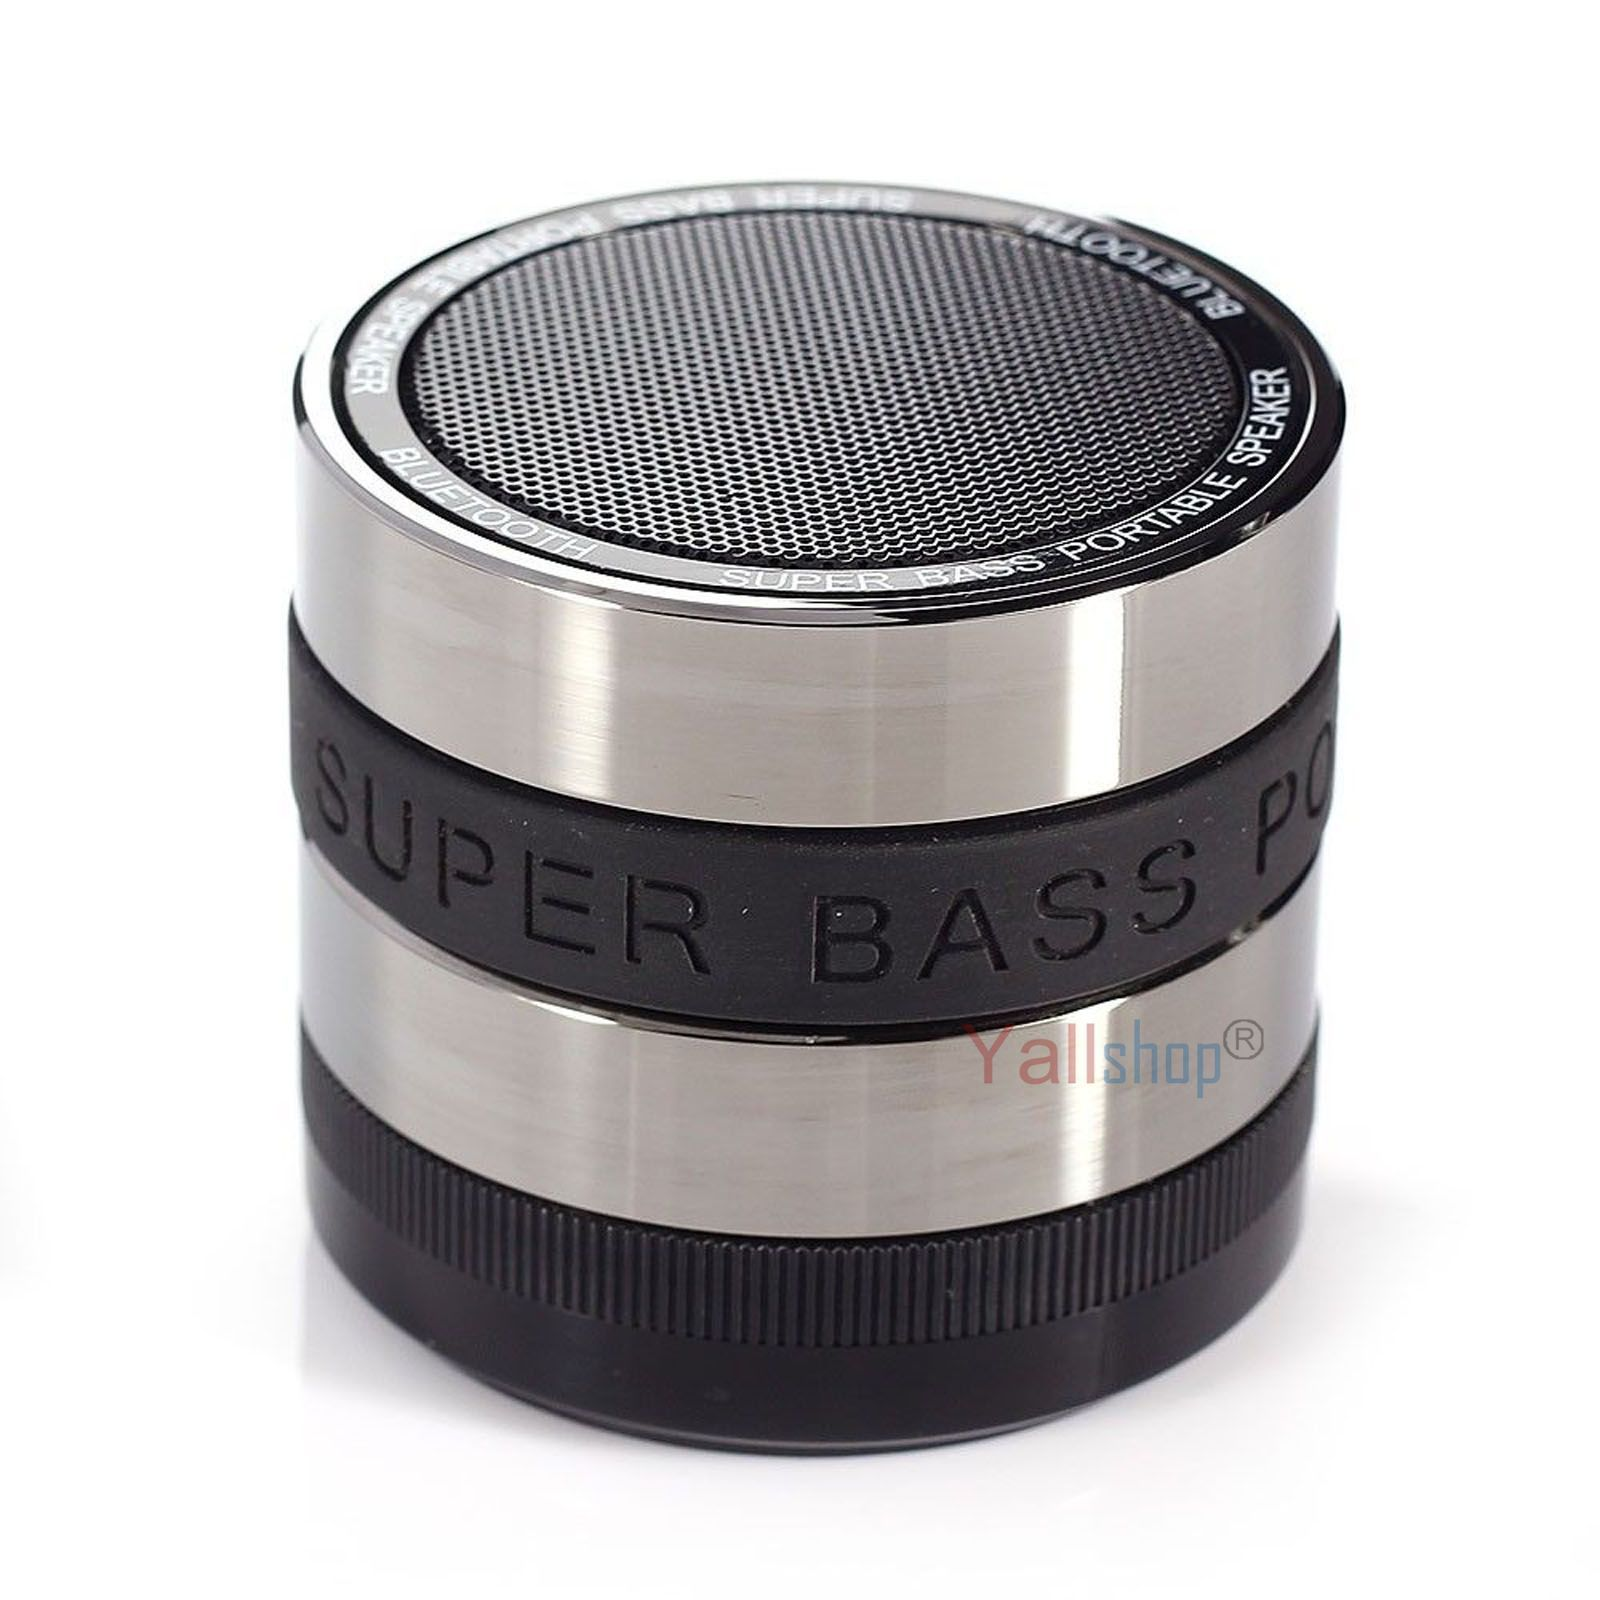
\includegraphics[height=4.0cm]{figures/standard-iphone-speaker.jpg}&
\includegraphics[height=3.5cm]{figures/standard-clock.jpg}\\
(a) Black Qi Standard Wireless Charging Charger Receiver Case For iPhone 5 5G & (b) Bluetooth Wireless Speaker Mini Portable Super Bass For iPhone & (c) Modern DIY Your Wall Clock Sticker Decoration Home Roman Numerals Silver SCY07\\
\end{tabular}
\end{center}
\end{table*}


\begin{table*}[t]
\caption{Examples of eBay interesting products. The highlighted keywords are not expected to co-occur in the context of the product.}
\label{tab:ebay-interesting-products}
\begin{center}
\begin{tabular}{LLL}
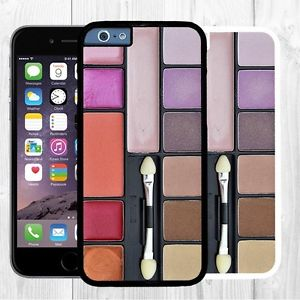
\includegraphics[height=3.5cm]{figures/eyeshadow-iphone-case.jpg}&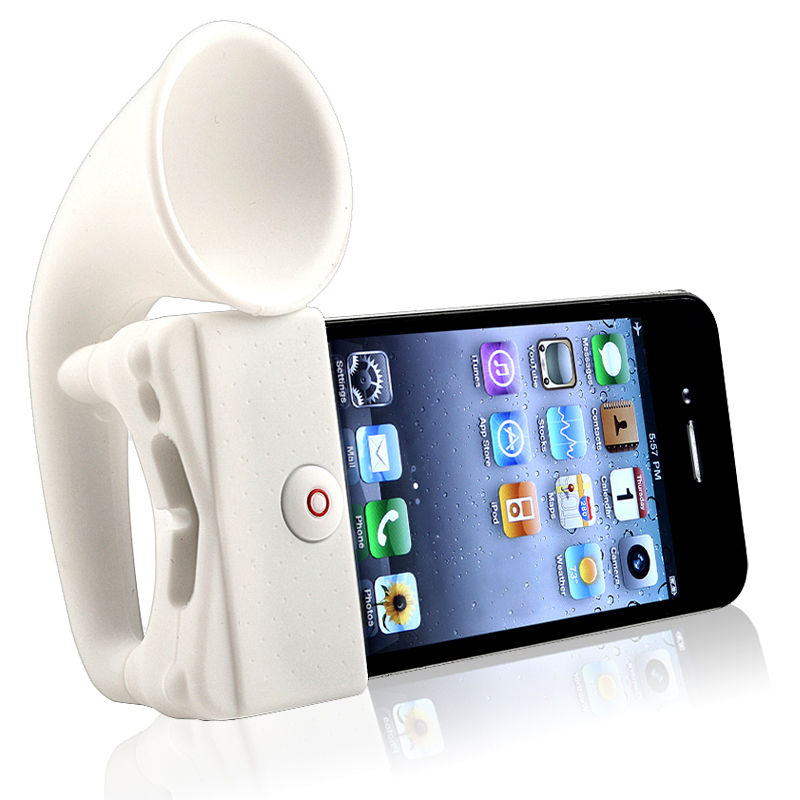
\includegraphics[height=4.5cm]{figures/horn-iphone-speaker.jpg}&
\includegraphics[height=4.0cm]{figures/geeky-clock.jpg}\\
(a) \textcolor{red}{{\bf Eyeshadow}} Palettes for \textcolor{red}{{\bf iPhone}} 6 case & (b) White Silicone \textcolor{red}{{\bf Horn}} Stand Speaker for Apple \textcolor{red}{{\bf iPhone}} 4/ 4S& (c) \textcolor{red}{{\bf Equation}} Wall \textcolor{red}{{\bf Clock}} Gifts for Math Gurus\\
\end{tabular}
\end{center}
\end{table*}